\documentclass[12pt, a4paper]{article}
\usepackage{xltxtra}

\usepackage{amsmath,amsfonts,amssymb,amsthm}
\usepackage{fontspec}
\defaultfontfeatures{Ligatures=TeX,Mapping=tex-text}
\setmainfont{CMU Serif}
\newfontfamily\cyrillicfont[Script=Cyrillic]{CMU Serif}
\setmonofont{CMU Typewriter Text}
\newfontfamily\cyrillicfonttt[Script=Cyrillic]{CMU Typewriter Text}
\setsansfont{CMU Sans Serif}
\newfontfamily\cyrillicfontsf[Script=Cyrillic]{CMU Sans Serif}

\usepackage{unicode-math}
\setmathfont{Latin Modern Math}

\usepackage{polyglossia}
\setmainlanguage[spelling=modern]{russian}
\setotherlanguage{english}
\setkeys{russian}{babelshorthands=true}

\usepackage[shortlabels]{enumitem}
\usepackage[russian,colorlinks,pagebackref]{hyperref}
\usepackage{listingsutf8}

\usepackage{fullpage}
\usepackage{color}
\usepackage{xcolor}
\usepackage{graphicx}
\usepackage{indentfirst}

\DeclareGraphicsExtensions{.pdf,.png,.jpg}
\graphicspath{{images/}}

\newtheorem{problem}{Задача}

\newenvironment{solution}
{\renewcommand\qedsymbol{$\blacksquare$}\begin{proof}[Решение]}
{\end{proof}}

\begin{document}
    \definecolor{dkgreen}{rgb}{0,0.6,0}
    \definecolor{gray}{rgb}{0.5,0.5,0.5}
    \definecolor{mauve}{rgb}{0.58,0,0.82}

    \newcommand{\problemset}[1]{

        \begin{center}
            \Large #1
        \end{center}
    }

    \newcommand{\defeq}{\overset{\mathrm{def}}{=\joinrel=}}

    \lstset{
        language=C++,                   % the language of the code
        basicstyle=\ttfamily\small,     % the size of the fonts that are used for the code
        backgroundcolor=\color{white},  % choose the background color. You must add \usepackage{color}
        numbers=none,                   % where to put the line-numbers
        numbersep=0pt,                  % how far the line-numbers are from the code
        frame=single,                   % adds a frame around the code
        framextopmargin=2pt,
        framexbottommargin=2pt,
        columns=fullflexible,
        rulecolor=\color{black!30},     % if not set, the frame-color may be changed on line-breaks within not-black text (e.g. comments (green here))
        tabsize=2,                      % sets default tabsize to 2 spaces
        showtabs=true,                  % show tabs within strings adding particular underscores
        showspaces=false,               % show spaces adding particular underscores
        keepspaces=true,
        showstringspaces=false,         % underline spaces within strings
        title=\lstname,                 % show the filename of files included with \lstinputlisting;
        escapeinside={\%*}{*)},         % if you want to add LaTeX within your code
        captionpos=b,                   % sets the caption-position to bottom
        breaklines=true,                % sets automatic line breaking
        breakatwhitespace=true,         % sets if automatic breaks should only happen at whitespace
        inputencoding=utf8,
        extendedchars=true,
        literate={*}{{\char42}}1 {-}{{\char45}}1,
        texcl=true,
        keywordstyle=\color{blue},      % keyword style
        commentstyle=\color{dkgreen},   % comment style
        stringstyle=\color{mauve},      % string literal style
    }

    \begin{tabbing}
\hspace{11cm} \= Студент: \= Беспалов В. A. \\
  \> Группа: \> M4160 \\
  \> Дата: \> \today
\end{tabbing}
\hrule
\vspace{1cm}

    \problemset{Домашнее задание}
\lstinputlisting[title={Определения для \href{https://jscoq.github.io/scratchpad.html}{Coq} - интерактивного средства доказательства теорем}]{proofs/Defs.v}

\begin{problem}
    Эквивалентны ли следующие факты?
\end{problem}

\begin{itemize}
    \item $f = \Theta(g)$
    \item $\exists c,  0 < c < +\infty : \lim\limits_{n \to +\infty} \frac{f(n)}{g(n)} = c$
\end{itemize}

\begin{solution}
    \leavevmode\vspace{1pt}
    \begin{enumerate}
        \item $f = \Theta(g) \Leftrightarrow f = O(g) \land f = \Omega(g)$

            Докажем эквивалентность. Определения:

            \begin{itemize}
                \item $f = \Theta(g) \defeq \exists N, c_1 > 0, c_2 > 0 : \forall n > N : c_1 \cdot g(n) \le f(n) \le c_2 \cdot g(n)$
                \item $f = O(g) \defeq \exists N, c > 0 : \forall n > N : f(n) \le c \cdot g(n)$
                \item $f = \Omega(g) \defeq \exists N, c > 0 : \forall n > N : c \cdot g(n) \le f(n)$
            \end{itemize}

            \begin{enumerate}
                \item Воспользуемся симметричностью операции $\land$:
                    \hfill \break
                    $f = \Theta(g) \Leftrightarrow f = \Omega(g) \land f = O(g)$

                \item Выполним подстановку:
                    \hfill \break
                    $\exists N, c_1 > 0, c_2 > 0 : \forall n > N : c_1 \cdot g(n) \le f(n) \le c_2 \cdot g(n) \Leftrightarrow c_1 \cdot g(n) \le f(n) \land f(n) \le c_2 \cdot g(n)$

                \item Таким образом:
                    \hfill \break
                    $c_1 \cdot g(n) \le f(n) \le c_2 \cdot g(n) \Leftrightarrow c_1 \cdot g(n) \le f(n) \le c_2 \cdot g(n)$

                    \leavevmode\vspace{1pt}
                    \lstinputlisting[title={Листинг доказательства}]{proofs/Task1.v}
                    \qedsymbol
            \end{enumerate}

        \item Воспользуемся определением нотаций через пределы:

            \begin{itemize}
                \item $f(n) = O(g(n)) \defeq \lim\limits_{n \to +\infty} \frac{f(n)}{g(n)} < +\infty$
                \item $f(n) = \Omega(g(n)) \defeq \lim\limits_{n \to +\infty} \frac{f(n)}{g(n)} > 0$
            \end{itemize}

            \begin{enumerate}
                \item Из пункта 1 следует:

                    $f(n) = \Theta(g(n)) \Leftrightarrow \lim\limits_{n \to +\infty} \frac{f(n)}{g(n)} < +\infty \land \lim\limits_{n \to +\infty} \frac{f(n)}{g(n)} > 0$

                \item Таким образом:

                    $f(n) = \Theta(g(n)) \Leftrightarrow 0 < \lim\limits_{n \to +\infty} \frac{f(n)}{g(n)} < +\infty$

                \item Иными словами:

                    $f(n) = \Theta(g(n)) \Leftrightarrow \exists c,  0 < c < +\infty : \lim\limits_{n \to +\infty} \frac{f(n)}{g(n)} = c$
            \end{enumerate}
    \end{enumerate}
\end{solution}


\begin{problem}
    Дайте ответ для двух случаев $\mathbb{N} \to \mathbb{N}$ и $\mathbb{N} \to \mathbb{R}_{>0}$:
\end{problem}

\begin{enumerate}[(a)]
    \item Если в определении $O$ опустить условие про $N$ (т.е. оставить
        просто $\forall n$), будет ли полученное определение эквивалентно
        исходному?
    \item Тот же вопрос про $o$.
\end{enumerate}

\begin{solution}
    \leavevmode\vspace{1pt}

    Отметим, что $\mathbb{N} \in \mathbb{R}_{>0}$, поэтому всё нижеперечисленное будет относиться как к $\mathbb{N}$, так и к $\mathbb{R}_{>0}$.

    \begin{enumerate}[(a)]
        \item Пример: для $f(n) = \sqrt{n^2 + 27n + 65}$ и $g(n) = n$ будет выполняться $f = O(g)$, потому что при $N = 5$ функция $f$ ограничена сверху функцией $3g$.
            Если убрать из исходного определения условие про существование $N$, то очевидно, что при $n \le 5$ ситуация будет обратной -- при сохранении $c = 3$ функция $3g$ будет ограничена сверху функцией $f$.
            Следовательно, модифицированное определение не эквивалентно исходному.

            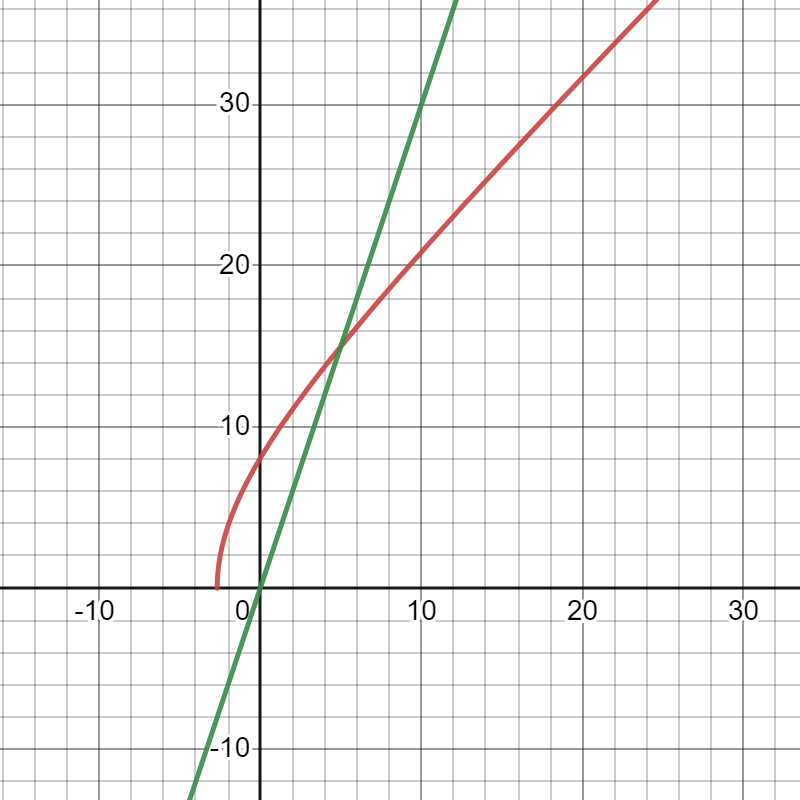
\includegraphics[scale=0.2]{Graph_1}

        \item Пример: для $f(n) = 9n$ и $g(n) = n^3$ будет выполняться $f = o(g)$.

            Докажем это. Определения:

            \begin{itemize}
                \item $f = o(g) \defeq \forall c > 0 : \exists N : \forall n > N : f(n) < c \cdot g(n)$
            \end{itemize}

            \begin{enumerate}[1.]
                \item Развернём отношение:
                    \hfill \break
                    $\forall c > 0 : \exists N : \forall n > N : 9n < c \cdot (n \cdot n \cdot n)$

                \item Воспользуемся ассоциативностью умножения:
                    \hfill \break
                    $\forall c > 0 : \exists N : \forall n > N : 9n < c \cdot n \cdot n \cdot n$

                \item Известно, что $n > 0$. Поделим обе части выражения на $n$:
                    \hfill \break
                    $\forall c > 0 : \exists N : \forall n > N : 9 < c \cdot n \cdot n$

                \item Известно, что $c > 0$. Поделим обе части выражения на $c$:
                    \hfill \break
                    $\forall c > 0 : \exists N : \forall n > N : \dfrac{9}{c} < n \cdot n$

                \item Извлечём квадратный корень из обеих частей выражения:
                    \hfill \break
                    $\forall c > 0 : \exists N : \forall n > N : \sqrt{\dfrac{9}{c}} < n$

                \item Теперь можно доказать существование $N$ для всех $c > 0$:
                    \hfill \break
                    $n > N \land \sqrt{\dfrac{9}{c}} < n \implies N \in [\sqrt{\dfrac{9}{c}}, +\infty)$

                    \leavevmode\vspace{1pt}
                    \lstinputlisting[title={Листинг доказательства}]{proofs/Task2.v}
                    \qedsymbol
            \end{enumerate}

            Если убрать из исходного определения условие про существование $N$, то очевидно, что при $n \le \sqrt{\dfrac{9}{c}}$ функция $g$ перестанет быть строго доминирующей над функцией $f$.
            Следовательно, модифицированное определение не эквивалентно исходному.
    \end{enumerate}
\end{solution}


\begin{problem}
    Продолжим отношение `$\preceq$' на функциях до отношения на классах эквивалентности по отношению эквивалентности `$\sim$', введённому на практике. Правда ли, что получится отношение \texttt{линейного порядка} (то есть $\forall f, g: (f \preceq g) \lor (g \preceq f)$)?
\end{problem}

\begin{solution}
    \leavevmode\vspace{1pt}
    \lstinputlisting[title={Листинг доказательства}]{proofs/Task3.v}
\end{solution}


\begin{problem}
    Докажите, или приведите контрпример:
    \begin{enumerate}[(a)]
        \item $g(n) = o(f(n)) \Rightarrow f(n) + g(n) = \Theta(f(n))$
        \item $f(n) = O(g(n)) \Leftrightarrow f(n) = o(g(n)) \lor f(n) = \Theta(g(n))$
    \end{enumerate}
\end{problem}

\begin{solution}
    \leavevmode\vspace{1pt}

    \begin{enumerate}[(a)]
        \item Выполним верификацию теоремы:
            \leavevmode\vspace{1pt}
            \lstinputlisting[title={Пункт (a). Листинг доказательства}]{proofs/Task4-1.v}
            \qedsymbol

        \item Приведем неудачную верификацию теоремы:
            \leavevmode\vspace{1pt}
            \lstinputlisting[title={Пункт (b). Листинг отмененного доказательства}]{proofs/Task4-2.v}

            Цель $(f = O(g) \rightarrow f = o(g)) \lor (f = O(g) \rightarrow f = \Theta(g))$ недостижима:

            \begin{itemize}
                \item При прохождении по левой ветке, доказать, что $\forall c > 0 : f(n) < c \cdot g(n)$, имея в контексте $\exists c > 0 : f(n) \le c \cdot g(n)$, не представляется возможным.

                \item При прохождении по правой ветке, доказать, что $c \cdot g(n) \le f(n)$, имея в контексте $f(n) \le c \cdot g(n)$, не представляется возможным.
            \end{itemize}
    \end{enumerate}
\end{solution}


\begin{problem}
    Решите рекурренту $T(n) = 3 T(\sqrt{n}) + \log_2 n$ (найдите точную оценку асимптотики и докажите). Здесь можно считать, что $T(n \le 1) = 1$.
\end{problem}

\begin{solution}
    \leavevmode\vspace{1pt}

    \begin{enumerate}
        \item $m \defeq \log_2{n} \rightarrow n = 2^{\log_2{n}} = 2^m$. Тогда: $T(2^m) = 3 T(2^{m / 2}) + m$
        \item $S(m) \defeq T(2^m) \rightarrow T(2^{m / 2}) = S(m / 2)$. Тогда: $S(m) = 3 S(m / 2) + m$
        \item Допустим, \( \exists m_0, c > 0, b > 0 : \forall m > m_0 : S(m) \le c \cdot m^{log_2{3}} - bm \).
            \begin{itemize}
                \item \( S(m) = 3 S(m / 2) + m \)
                \item \( 3 S(m / 2) + m \le 3 \left( c \cdot (m / 2)^{log_2{3}} - b \cdot (m / 2) \right) + m \)
                \item \( 3 \left( c \cdot (m / 2)^{log_2{3}} - b \cdot (m / 2) \right) + m = 3c \cdot \dfrac{m^{log_2{3}}}{2^{log_2{3}}} - 3b \cdot (m / 2) + m \)
                \item \( 3c \cdot \dfrac{m^{log_2{3}}}{2^{log_2{3}}} - 3b \cdot (m / 2) + m = c \cdot m^{log_2{3}} - bm - (b / 2 - 1)m \)
                \item \( (b / 2 - 1)m \ge 0 \rightarrow c \cdot m^{log_2{3}} - bm - (b / 2 - 1)m \le c \cdot m^{log_2{3}} - bm \)
            \end{itemize}
        \item Следовательно: \( S(m) = O(m^{log_2{3}}) \rightarrow T(n) = O((log_2{n})^{log_2{3}}) \)
    \end{enumerate}
\end{solution}


\begin{problem}
    Заполните табличку и поясните (особенно строчки 4 и 7):
    $$
    \begin{array}{|cc|c|c|c|c|c|}
        \hline
        A & B & O & o & \Theta & \omega & \Omega \\
        \hline
        n & n^2 & + & + & - & - & - \\
        \log^k n & n^{\xi} & + & + & - & - & - \\
        n^k & c^n & + & + & - & - & - \\
        \sqrt{n} & n^{\sin n} & - & - & - & - & - \\
        2^n & 2^{n \slash 2} & - & - & + & + & - \\
        n^{\log m} & m^{\log n} & + & - & + & - & + \\
        \log (n!) & \log(n^n) & + & - & + & - & + \\
        \hline
    \end{array}
    $$
    Здесь все буквы, кроме $n$, -- положительные константы.
\end{problem}


\subsection*{Дополнительные задачи}

\begin{problem}
    Считайте здесь, что функции здесь $\mathbb{N} \to \mathbb{N}$ и что $\forall n : f(n) > 1 \land g(n) > 1$.
    \begin{enumerate}[(a)]
        \item $f(n) = O(g(n)) \Rightarrow \log f(n) = O(\log g(n))$?
        \item $f(n) = O(g(n)) \Rightarrow 2^{f(n)} = O(2^{g(n)})$?
    \end{enumerate}
\end{problem}

\begin{solution}
    \ldots
\end{solution}


\begin{problem}
    Упорядочьте функции по скорости роста и обозначьте неравенства между соседями.
    Укажите, в каких неравенствах $f = o(g)$, а в каких $f = \Theta(g)$
    $$
    \begin{array}{cccccc}
        \log(\log^* n) & 2^{log^* n} & (\sqrt{n})^{\log n} & n^2 & n! & (\log n)! \\
        (3 \slash 2)^n & n^3 & \log^2 n & \log n! & 2^{2^n} & n^{1 \slash \log n} \\
        \ln \ln n & \log^* n & n \cdot 2^n & n^{\log \log n} & \ln n & 1 \\
        2^{\ln n} & (\log n)^{\log n} & e^n & 4^{\log n} & (n + 1)! & \sqrt{\log n} \\
        \log^* \log n & 2^{\sqrt{2 \log n}} & n & 2^n & n \log n & 2^{2^{n + 1}}
    \end{array}
    $$
    Примечание: $\log^*(n) = \left\{
        \begin{array}{ll}
            0 & \texttt{ если } n \leq 1;\\
            1 + \log^*(\log n) & \texttt{ иначе.}
        \end{array}
        \right.$
\end{problem}

\begin{solution}
    \ldots
\end{solution}


\clearpage

\end{document}
